\documentclass{aa}

\usepackage{graphicx}
\usepackage{txfonts}
\usepackage{booktabs}
\usepackage{xcolor}

\newcommand{\todo}[1]{\textcolor{red}{TODO: #1}}
\newcommand{\simg}{\ensuremath{[\mathrm{Si}/\mathrm{Mg}]}}
\newcommand{\mgfe}{\ensuremath{[\mathrm{Mg}/\mathrm{Fe}]}}
\newcommand{\mh}{\ensuremath{[\mathrm{M}/\mathrm{H}]}}

\begin{document}

\title{A brief early Si-rich enrichment channel in compact relic galaxy formation}

\author{Tereza~TODO\inst{1}
\and Collaborators~TODO\inst{2}}

\institute{
TODO: Institute 1
\and
TODO: Institute 2
}

\abstract
{Compact relic galaxies provide stringent tests of early chemical enrichment because their stellar populations formed rapidly and experienced little subsequent dilution. NGC~1277 is especially interesting because Eftekhari-style near-infrared (NIR) analysis suggests high silicon relative to magnesium, while a successful clean relic model predicts much lower \simg.}
{We test whether a short early Si-rich enrichment episode can raise the model \simg\ while preserving the relic fit in stellar mass, metallicity, \mgfe, and mass-to-light ratio.}
{We summarize copied-code yield-channel tests built on an environment-dependent, time-variable galaxy-wide IMF model, using IGIMF/GalIMF as the computational machinery/tool. We compare clean, pre-enriched, mixed PopIII/PISN-like, and timed PopIII/PISN-like Si-rich enrichment experiments. We also test E-MILES NIR-local weighting as a first-order bridge to the observed NIR indices.}
{The clean NGC~1277-like baseline has code-light \simg=0.058, and E-MILES NIR-local weighting raises this only to \simg=0.075. The best accepted timed model, \texttt{timed\_s0\_d40\_m170\_f0p35\_e1p00}, reaches E-MILES NIR-local \simg=0.499 while remaining within the adopted relic-fit tolerance box: $\Delta\mh=+0.095$, $\Delta\mgfe=-0.070$, $\Delta\log M=+0.137$, and $\Delta\log M/L=+0.053$. Extending the same channel to 50 Myr reaches $\simg_{\rm NIR}\simeq0.523$ but is rejected because metallicity, \mgfe, and stellar mass degrade.}
{The current framework reaches the lower high-Si regime but not the nominal Eftekhari-like value near $\simg\simeq0.67$ without additional yield selectivity, localized enrichment, or NIR abundance-response systematics. The reported values are chemical-evolution abundance proxies, not full spectral-index abundance inferences.}

\keywords{galaxies: abundances -- galaxies: elliptical and lenticular, cD -- galaxies: evolution -- galaxies: stellar content -- stars: luminosity function, mass function}

\maketitle

\section{Introduction}

Compact relic galaxies provide a stringent test of early galaxy formation because they preserve old, dense stellar populations with limited subsequent dilution. NGC~1277 is a particularly useful case: a successful relic model must reproduce stellar mass, metallicity, high \mgfe, and mass-to-light ratio while remaining consistent with a rapid formation history.

The remaining tension is silicon. Eftekhari-style NIR index analysis suggests a high silicon abundance relative to magnesium, with a practical lower high-Si comparison near $\simg\simeq0.4$ and a nominal NGC~1277 comparison near $\simg\simeq0.67$. The clean chemical-evolution relic model predicts a much lower \simg. This paper draft asks whether a controlled early Si-rich enrichment channel can raise \simg\ while preserving the relic fit.

We use the phrase environment-dependent, time-variable galaxy-wide IMF model for the science framework. IGIMF/GalIMF is used only for the computational machinery/tool that evaluates the galaxy-wide IMF. The yield-channel experiments described here are copied-code tests and are not production-code replacements.

\section{Baseline relic model}

The clean copied-code NGC~1277 baseline has $\log M_\star=11.082$, light-weighted \mh\ or $[Z/X]=0.262$, \mgfe=0.422, $[\mathrm{Si}/\mathrm{Fe}]=0.480$, \simg=0.058, and $M/L=29.374$ in internal code luminosity units. This model remains the reference for all relic-fit deltas.

The baseline is successful as a relic fit but not as a high-Si model. E-MILES NIR-local weighting raises the clean baseline only to \simg=0.075. Therefore, the discrepancy is not explained by a simple change from the internal code luminosity weighting to NIR-local flux weighting.

Table~\ref{tab:key_models} summarizes the key models used throughout the draft.

\begin{table*}
\centering
\caption{Key NGC~1277 Si/Mg model comparison. Values are copied from \texttt{final\_relic\_simg\_key\_models.csv}. Blank entries indicate quantities not available in that compact table.}
\label{tab:key_models}
\begin{tabular}{llrrrrrl}
\toprule
Model & Type & Code-light \simg & NIR \simg & $\Delta\mh$ & $\Delta\mgfe$ & $\Delta\log M$ & Status \\
\midrule
\texttt{clean\_baseline} & Clean relic baseline & 0.058 & 0.075 & 0.000 & 0.000 & 0.000 & accepted \\
\texttt{mixed\_popiii170\_v5\_f0.1} & Mild mixed channel & 0.158 & 0.311 & -- & -- & -- & accepted; Si/Mg too low \\
\texttt{timed\_s0\_d40\_m170\_f0p35\_e1p00} & Best accepted timed & 0.372 & 0.499 & +0.095 & -0.070 & +0.137 & accepted \\
\texttt{timed\_s0\_d50\_m170\_f0p35\_e1p00} & First rejected timed & 0.410 & 0.523 & +0.113 & -0.085 & +0.168 & rejected \\
\texttt{mixed\_popiii170\_v5\_c100\_z1\_f0.3} & Highest rejected mixed & -- & 0.574 & +0.166 & -0.142 & +0.268 & rejected \\
\bottomrule
\end{tabular}
\end{table*}


\section{Methods}

\subsection{Environment-dependent time-variable galaxy-wide IMF model}

The underlying science framework is an environment-dependent, time-variable galaxy-wide IMF model. IGIMF/GalIMF is used as the computational machinery/tool for the galaxy-wide IMF. In the tests described here, the NGC~1277 relic best-fit parameters are held fixed unless stated otherwise; the scans perturb the enrichment channel rather than refitting the full model.

\subsection{Chemical-evolution setup and standard yields}

The baseline follows the Nomoto-family relic chemical-evolution setup. The analysis tracks surviving stellar mass, light-weighted metallicity proxy, light-weighted \mgfe, $[\mathrm{Si}/\mathrm{Fe}]$, \simg, and internal $M/L$. The current light-weighted abundances are chemical-evolution abundance proxies. They are not full spectral-index abundance inferences.

\subsection{PopIII/PISN-like Si-rich yield-channel tests}

The Si-rich experiments are copied-code yield-channel tests. The mixed PopIII/PISN-like channel is controlled by opt-in environment variables and uses copied yield tables. The representative yield mass used by the current best model is $170\,M_\odot$, but the exact yield table and row remain a manuscript TODO.

\begin{table}
\centering
\caption{Yield-channel parameters for the compact model set. The PopIII/PISN-like mass, fraction, and timing describe copied-code yield-channel tests, not production-code replacements.}
\label{tab:yield_parameters}
\begin{tabular}{lrrrr}
\toprule
Model class & Start & Duration & Mass & Fraction \\
 & Myr & Myr & $M_\odot$ & \\
\midrule
Clean baseline & -- & -- & -- & 0.00 \\
Mild mixed channel & 0 & 30 & 170 & 0.10 \\
Best accepted timed & 0 & 40 & 170 & 0.35 \\
First rejected timed & 0 & 50 & 170 & 0.35 \\
Highest rejected mixed & 0 & 100 & 170 & 0.30 \\
\bottomrule
\end{tabular}
\tablefoot{The exact yield file/table row for the representative $170\,M_\odot$ PopIII/PISN-like channel remains a TODO before manuscript use.}
\end{table}


\subsection{E-MILES NIR-local weighting and index comparison}

E-MILES BaSTI baseFe bimodal SSP spectra were used in two ways. First, NIR-local fluxes around MgI~1.18, SiI~1.20, and SiI~1.59 were used to reweight stellar generations and recompute abundance averages. Second, public baseFe SSP spectra were measured for Eftekhari-style pseudo-equivalent-width indices, including velocity broadening to $\sigma=440\,\mathrm{km\,s^{-1}}$.

These tests do not provide abundance-variable response functions. They test flux weighting and baseline SSP/index behavior, not an independent inference of $[\mathrm{Si}/\mathrm{Fe}]$ or \mgfe.

\subsection{Model acceptance criteria}

\begin{table}
\centering
\caption{Adopted relic-fit acceptance criteria and comparison to the best accepted and first rejected timed models.}
\label{tab:acceptance}
\begin{tabular}{lrrr}
\toprule
Quantity & Tolerance & Best accepted & First rejected \\
\midrule
$|\Delta\mh|$ & $\leq 0.10$ dex & +0.095 & +0.113 \\
$|\Delta\mgfe|$ & $\leq 0.08$ dex & -0.070 & -0.085 \\
$|\Delta\log M|$ & $\leq 0.15$ dex & +0.137 & +0.168 \\
$|\Delta\log M/L|$ & $\leq 0.15$ dex & +0.053 & +0.072 \\
\bottomrule
\end{tabular}
\tablefoot{The best accepted model is \texttt{timed\_s0\_d40\_m170\_f0p35\_e1p00}; the first rejected model is \texttt{timed\_s0\_d50\_m170\_f0p35\_e1p00}.}
\end{table}


\section{Model tests}

\subsection{Clean baseline}

The clean baseline has code-light \simg=0.058 and E-MILES NIR-local \simg=0.075. It remains far below both the lower high-Si comparison near $\simg\simeq0.4$ and the nominal value near $\simg\simeq0.67$.

\subsection{Pre-enriched initial gas}

The pre-enriched initial-gas scan imposed initial \simg\ offsets from 0.0 to 0.8 while keeping the initial reservoir very metal-poor and changing only Si. The final stellar \simg\ remains near 0.058 in all cases. The initial signal is diluted, so simple low-metallicity Si pre-enrichment is insufficient.

\subsection{Two-component light mixing}

A two-component toy model mixed abundance ratios in linear Si/Mg space. A mild \simg=0.158 component cannot reach the nominal target: it would require 1194\% of the light for \simg=0.67. Even a \simg=0.5 component requires 175\% of the light for the nominal target. A localized interpretation therefore requires the relevant NIR light to be dominated by a component already near the target.

\subsection{Mixed PopIII/PISN-like enrichment}

The mild mixed model \texttt{mixed\_popiii170\_v5\_f0.1} raises code-light \simg\ to 0.158 and E-MILES NIR-local \simg\ to about 0.311. This is chemically useful but still below the lower high-Si regime.

Aggressive mixed-channel models can reach higher Si/Mg. For example, \texttt{mixed\_popiii170\_v5\_c100\_z1\_f0.3} reaches E-MILES NIR-local \simg=0.574, but it fails through excessive metallicity, low \mgfe, and high stellar mass. These models are sensitivity tests rather than accepted solutions.

\subsection{Timed early Si-rich enrichment}

The timed local-refinement scan finds a narrow accepted boundary. Earlier and shorter channels can raise \simg\ without destroying the relic fit. Longer or stronger channels push \simg\ higher but couple into total metallicity, \mgfe, and mass.

\section{Results}

\subsection{Best accepted model}

The best accepted model is \texttt{timed\_s0\_d40\_m170\_f0p35\_e1p00}. It starts at 0 Myr, lasts 40 Myr, uses representative $170\,M_\odot$ PopIII/PISN-like yields, has fraction 0.35, and assumes full mixing efficiency.

It reaches code-light \simg=0.372 and E-MILES NIR-local \simg=0.499. Its relic-fit deltas are $\Delta\mh=+0.095$, $\Delta\mgfe=-0.070$, $\Delta\log M=+0.137$, and $\Delta\log M/L=+0.053$. This is final-enough for discussion and lies within the adopted relic-fit tolerance box, but it is a boundary solution.

\begin{figure}
\centering
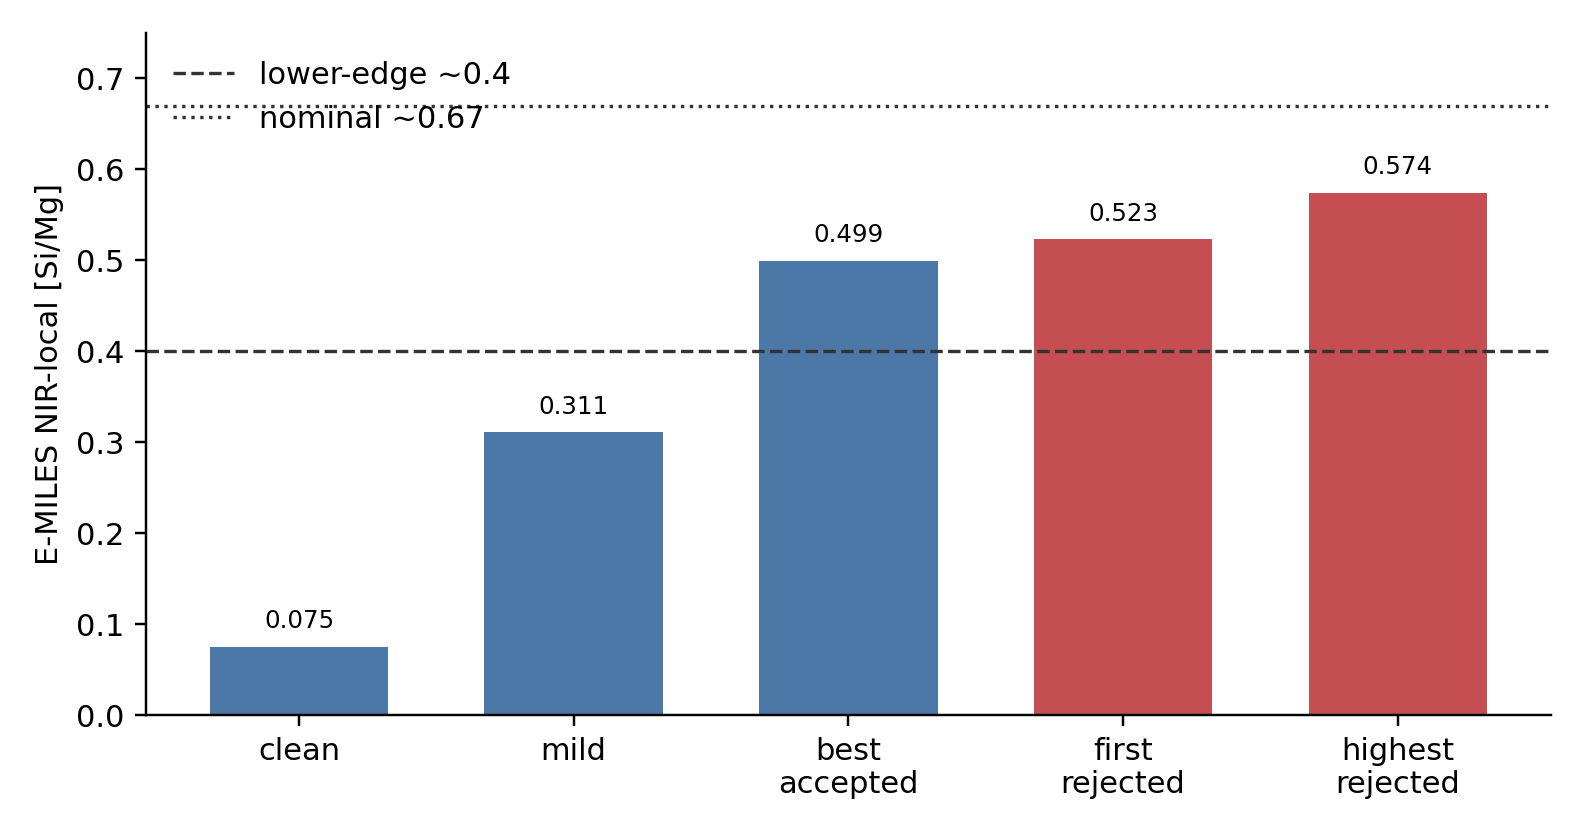
\includegraphics[width=\columnwidth]{figures/final_relic_simg_key_models.png}
\caption{Current key model comparison from the lightweight analysis products. The clean baseline stays at low \simg, while the best accepted timed Si-rich enrichment model reaches the lower high-Si regime. This figure should be remade in final A\&A style before submission.}
\label{fig:key_models}
\end{figure}

\subsection{First rejected higher-Si/Mg model}

The matched 50 Myr counterpart, \texttt{timed\_s0\_d50\_m170\_f0p35\_e1p00}, reaches E-MILES NIR-local $\simg\simeq0.523$, but is rejected. Its deltas are $\Delta\mh=+0.113$, $\Delta\mgfe=-0.085$, $\Delta\log M=+0.168$, and $\Delta\log M/L=+0.072$. The failures are total metallicity, \mgfe, and stellar mass; $M/L$ is less restrictive.

\subsection{Failure modes}

The high-Si failure modes are coupled. Raising Si/Mg by increasing or extending the mixed channel changes the integrated metal budget, depresses \mgfe, and shifts stellar mass. A successful enrichment channel must be Si-selective, localized, short-lived, or spectrally/aperture-weighted in a way that affects the NIR indices more than the whole one-zone relic.

% TODO figure placeholder:
% \begin{figure}
% \centering
% \includegraphics[width=\columnwidth]{figures/simg_pareto_failure_modes.pdf}
% \caption{Planned Si/Mg versus relic-fit degradation plot. Source tables: constrained_simg_local_refinement_v1.csv and high_simg_failure_modes_v1.csv.}
% \label{fig:pareto}
% \end{figure}

\subsection{Why NIR weighting alone is insufficient}

E-MILES NIR-local weighting increases the clean baseline by only 0.018 dex, from \simg=0.058 to about 0.075. It helps only when a chemically Si-rich population already exists. Therefore, weighting alone does not explain the baseline discrepancy.

% TODO figure placeholder:
% \begin{figure}
% \centering
% \includegraphics[width=\columnwidth]{figures/emiles_nir_weighting_effect.pdf}
% \caption{Planned comparison of current code-light and E-MILES NIR-local \simg\ values. Source table: emiles_nir_flux_weighted_abundances_v1.csv.}
% \label{fig:emiles_weighting}
% \end{figure}

\subsection{Normal ETG control sequence}

The NGC~1277 experiment needs a control population: normal early-type galaxies should not preserve the same strong Si-rich signature as a compact relic. We therefore compare the relic-strength channel with a weak/moderate fixed diagnostic sequence for ETG models calibrated to the mass--metallicity and mass--\mgfe\ relations. These tests are copied-code fixed diagnostics, not new optimizations. M1e9, M1e10, and M1e11 use current total-mass ETG rows as upper-limit controls, while M1e12 uses the validated $f_{\rm core}=0.8$ core model.

\begin{table*}
\caption{Weak/moderate PopIII/PISN-like Si-rich control sequence for fixed ETG diagnostics.}
\label{tab:weakmod_etg_sequence}
\centering
\begin{tabular}{lccccc}
\toprule
Mass & Clean & 20 Myr, $f=0.10$ & 40 Myr, $f=0.10$ & 20 Myr, $f=0.20$ & 40 Myr, $f=0.20$ \\
\midrule
M1e9  & 0.192 & 0.246 & 0.277 & 0.293 & 0.347 \\
M1e10 & 0.147 & 0.178 & 0.197 & 0.207 & 0.242 \\
M1e11 & 0.093 & 0.113 & 0.126 & 0.132 & 0.155 \\
M1e12 & 0.074 & 0.129 & 0.160 & 0.175 & 0.229 \\
\bottomrule
\end{tabular}
\tablefoot{Entries are chemical-evolution abundance proxies for \simg. M1e9 is treated as a low-mass upper-limit diagnostic rather than a normal massive ETG anchor. The M1e12 row uses the validated $f_{\rm core}=0.8$ core model; the lower-mass rows use existing total-mass fixed ETG diagnostics.}
\end{table*}


\begin{figure}
\centering
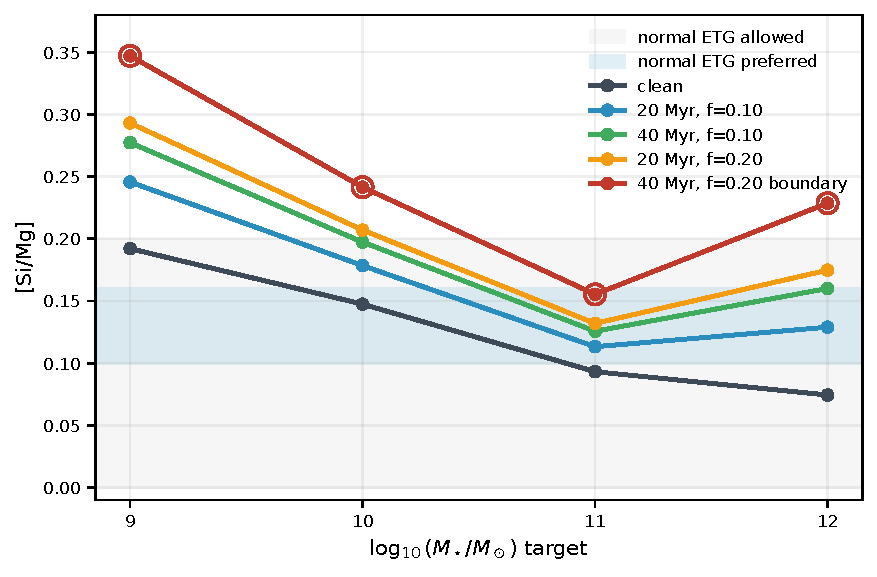
\includegraphics[width=\columnwidth]{figures/weakmod_etg_simg_sequence.pdf}
\caption{Weak/moderate Si-rich fixed diagnostic sequence for ETG controls. The conservative normal-ETG channel is the 20 Myr, $f=0.10$ case. M1e9 starts close to the upper normal \simg\ range and is therefore treated as a low-mass upper-limit diagnostic.}
\label{fig:weakmod_sequence}
\end{figure}

\begin{figure}
\centering
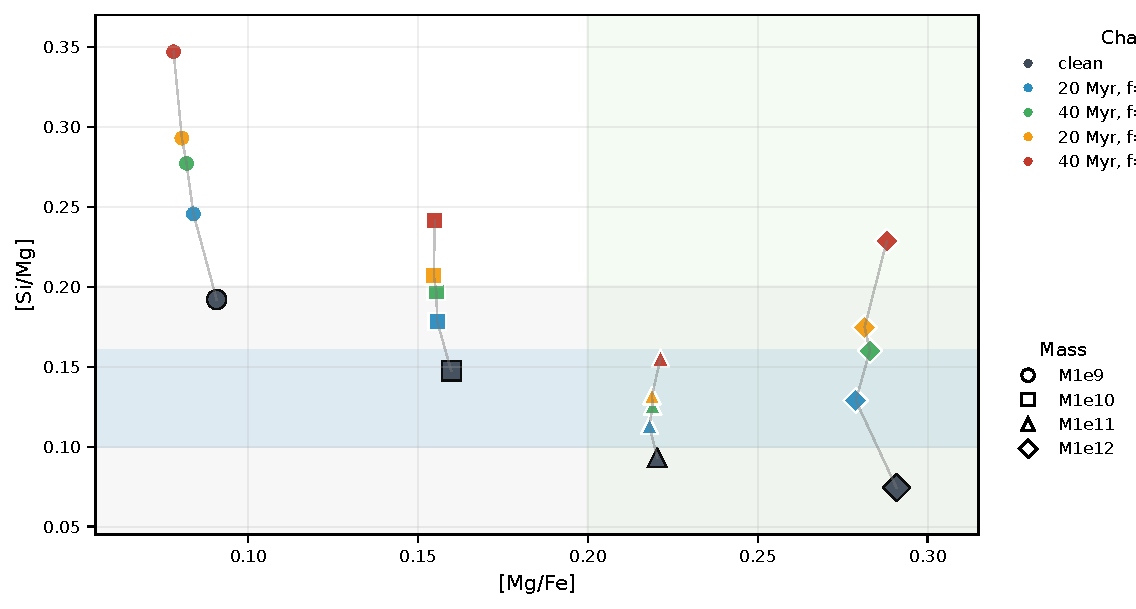
\includegraphics[width=\columnwidth]{figures/weakmod_etg_simg_vs_mgfe.pdf}
\caption{Control-sequence \simg\ versus \mgfe. The models preserve the calibration role of \mgfe\ while \simg\ separates the strength of preserved early Si-rich enrichment.}
\label{fig:weakmod_simg_mgfe}
\end{figure}

The safest normal-ETG preserved Si-rich channel is the 20 Myr, $f=0.10$ case. It remains compatible for M1e10, M1e11, and M1e12 while modifying \simg\ without breaking the stored mass, metallicity, and \mgfe\ calibration. The 40 Myr, $f=0.20$ case is best treated as an upper-normal or boundary case. The relic-strength $f=0.35$ channel is therefore reserved for NGC~1277-like high-preservation systems rather than normal ETG calibration.

\begin{figure}
\centering
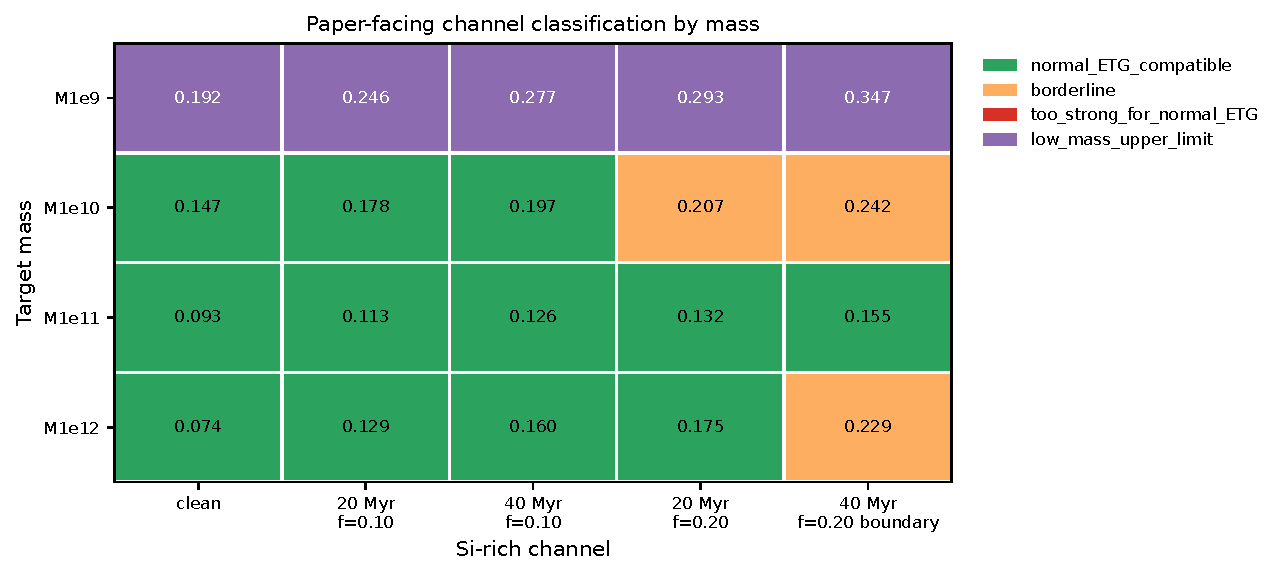
\includegraphics[width=\columnwidth]{figures/weakmod_allowed_channel_strength_by_mass.pdf}
\caption{Paper-facing classification of weak/moderate Si-rich channels by mass. The classification uses the multi-constraint calibration: stellar mass, metallicity, \mgfe, and whether \simg\ is in or can be diluted into the normal ETG locus with an old alpha-enhanced envelope.}
\label{fig:weakmod_allowed_strength}
\end{figure}

\begin{figure}
\centering
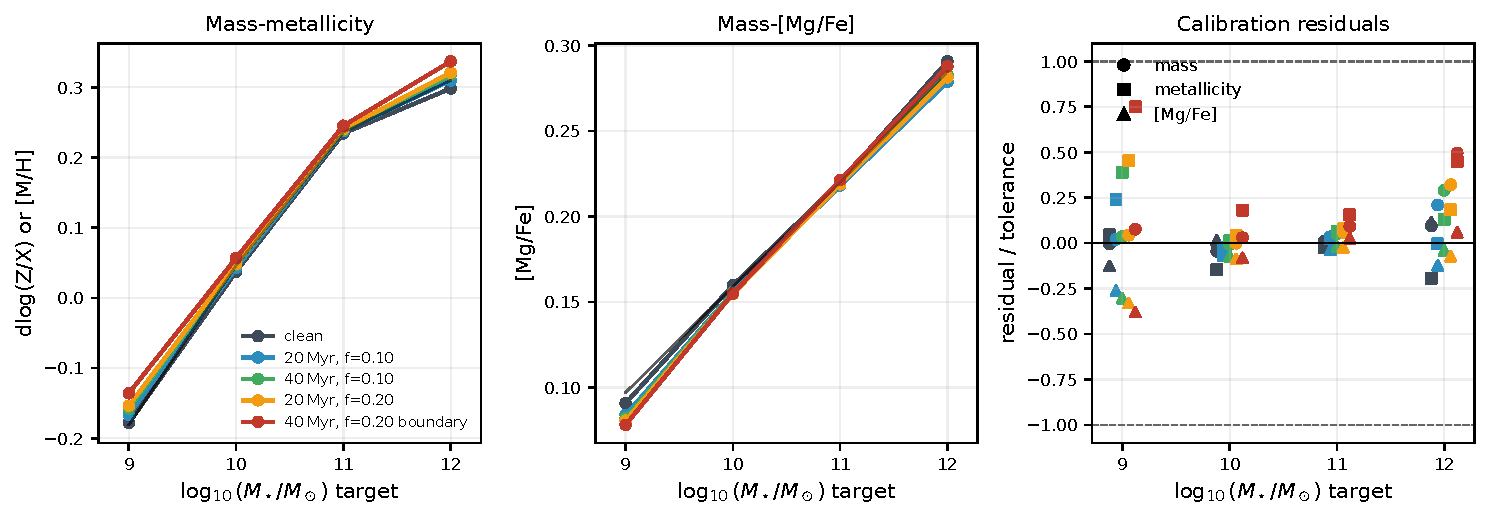
\includegraphics[width=\columnwidth]{figures/weakmod_mass_metallicity_mgfe_validation.pdf}
\caption{Mass--metallicity and mass--\mgfe\ validation for the weak/moderate control sequence. Accepted channels preserve the global ETG calibration while changing \simg.}
\label{fig:weakmod_validation}
\end{figure}

\section{Discussion}

\subsection{Physical interpretation}

A brief early Si-rich channel can explain the lower high-Si regime without immediately breaking the relic fit. The accepted model suggests enrichment confined to the first few tens of Myr, before the model accumulates too much total metal mass or suppresses \mgfe\ beyond the accepted limit.

\subsection{Si/Mg, Mg/Fe, and relicness}

Relicness should correlate robustly with \mgfe: old compact relics form rapidly and avoid late Fe-rich dilution. Si/Mg is a more conditional relicness tracer. It may correlate with relicness only if an early Si-rich channel operated and if later accreted or extended star formation did not dilute the signal.

\subsection{Why normal ETGs may dilute toward ordinary Si/Mg}

Normal early-type galaxies can build more extended stellar populations through longer star-formation histories, mergers, and accretion. Those later populations can dilute an early high-Si component in both mass and light, pushing integrated \simg\ toward more ordinary values even if the earliest compact core was Si-rich.

\subsection{Caveats about NIR abundance-response calibration}

The model values are chemical-evolution abundance proxies, not full spectral-index inferences. The E-MILES tests use baseFe SSP spectra for flux weighting and baseline index measurement, but not abundance-variable response functions. A publication-level comparison to Eftekhari-style $[\mathrm{Si}/\mathrm{Fe}]$, \mgfe, and \simg\ needs response-calibrated SiI and MgI NIR modeling at the appropriate velocity dispersion and aperture.

\section{Conclusions}

We summarize copied-code yield-channel tests of whether an NGC~1277-like compact relic can reproduce high NIR-inferred \simg\ while preserving the relic fit.

\begin{enumerate}
\item The clean NGC~1277-like relic baseline does not reach high Si/Mg: code-light \simg=0.058 and E-MILES NIR-local \simg=0.075.
\item Available abundance reweighting and E-MILES NIR-local weighting do not rescue the clean baseline.
\item Simple pre-enriched initial gas is diluted and fails to leave a high final stellar Si/Mg signal.
\item Mild mixed PopIII/PISN-like enrichment helps but remains below the lower high-Si regime.
\item The best accepted timed model, \texttt{timed\_s0\_d40\_m170\_f0p35\_e1p00}, reaches E-MILES NIR-local \simg=0.499 within the adopted relic-fit tolerance box.
\item The first higher-Si timed counterpart reaches $\simg\simeq0.523$ but is rejected because it degrades metallicity, \mgfe, and stellar mass.
\item The current framework reaches the lower high-Si regime but not nominal $\simg\simeq0.67$ without more Si-selective yields, localized enrichment, or revised NIR abundance-response interpretation.
\end{enumerate}

\begin{acknowledgements}
TODO: Add funding, software, and collaborator acknowledgements. This draft uses copied-code yield-channel tests and lightweight analysis products generated from the local NGC~1277 Si/Mg project directory.
\end{acknowledgements}


\bibliographystyle{aa}
\bibliography{references}

\end{document}
